\documentclass{article}
\usepackage{graphicx} % Required for inserting images
\usepackage{mathrsfs, geometry}
\geometry{a4paper,top=2cm,bottom=2cm,left=3cm,right=1cm}

\usepackage[T2A]{fontenc}
\usepackage[cp1251]{inputenc} %% Win  (for new docs)
%\usepackage[cp866]{inputenc} %% DOS  (for old docs)
\usepackage[russian]{babel}

\usepackage{indentfirst}
\usepackage{epsfig,amssymb,latexsym,amsmath,euscript,epic,eepic,color, graphics}
\usepackage{xcolor}
\usepackage{environ}
\NewEnviron{myequation}{%
\begin{equation}
\centerline{\scalebox{1.3}{$\BODY$}}
\end{equation}
}

\title{Methods of numerical solutions of differential equations}





\date{}

\begin{document}

\large %%title page
 \pagestyle{empty}
\begin{center}
{FEDERAL STATE AUTONOMOUS EDUCATIONAL INSTITUTION\\
FOR HIGHER EDUCATION\\
NATIONAL RESEARCH UNIVERSITY HIGHER SCHOOL OF ECONOMICS}\\
{\textit {Faculty of Informatics, Mathematics, and Computer Science}}\\
\end{center}
\vspace{30mm}
\begin{center}
{\Large Nikita A. Mezentsev}
\end{center}
\begin{center}
{\Large \bf On Numerical Modelling of Solutions of Differencial Equation}
\end{center}

\begin{center}
{\Large Master thesis}
\end{center}
\begin {center}
{\Large Field of Study: 01.04.01 Mathematics}
\end{center}
\begin{center}
{\Large Master's Programme Mathematics}
\end{center}

\vspace{10mm}
\begin{center}
\end{center}


\vspace{5mm}

\begin{flushright}
{\Large               Supervisor\\ Candidate of Sciences\\
Associate Professor\\ Gurevich E. Ya.}\\
\end{flushright}

\vspace{90mm}
\begin{center}
Nizhny Novgorod, 2023
\end{center}

\pagebreak

\renewcommand\contentsname{The Table of Contents} %%% renaming the Table of Contents
\sloppy
\normalfont
\tableofcontents

\pagebreak

\section{Introduction}
In this paper, the problem of incorrect differential equations' solution by numerical methods is considered. Numerical solutions of differential equations are common among students. They rely on the answers of web applications without thinking that it can be wrong. So, the purpose of the course work is to create an application with hints for students to pay their attention to the difference between numerical and accurate solutions and allow them to explore the causes of mistakes. To be more exact, multiple differential equations have been solved with Euler's and Runge-Kutta methods and then the results have been compared with accurate solution. To demonstrate the difference between resulting curves, Python programming language was used. It includes a module, called SymPy, which allows to solve differential equation and then generate points using an accurate solution. However, this module cannot cope with some equations and this problem is described in the paper. Actually, 'matplotlib' module gave an opportunity to illustrate curves of numerical and accurate solutions. To prevent misunderstandings of students, which analyzing specific differential equations, an applications with graphical user interface has been implemented. Python language includes PyQT5 framework, which allows to connect command application with buttons of GUI and assess results after its execution. Student would be able to observe how numerical methods can be wrong. Accurate solutions of the specific differential equations have been obtained manually and then a solving algorithm has been integrated in the application. Students have an opportunity to choose random initial condition and the number of steps for numerical methods for convenient analysis. The application is described in more details in this paper.
\par Modern applications, which provide an interface of solving differential equations numerically, show plot with errors. Sometimes description of methods and location of errors are not specified. Therefore, students take this solutions for the truth and think that it is the same (or similar) as an accurate solution. Lower on the image, the output of the differential equations' solver application contains an error which are considered in this paper. The program, which was required to implement, should show students an accurate solutions and errors of numerical methods for analysis and understanding.
\vspace{15mm}
\begin{center}
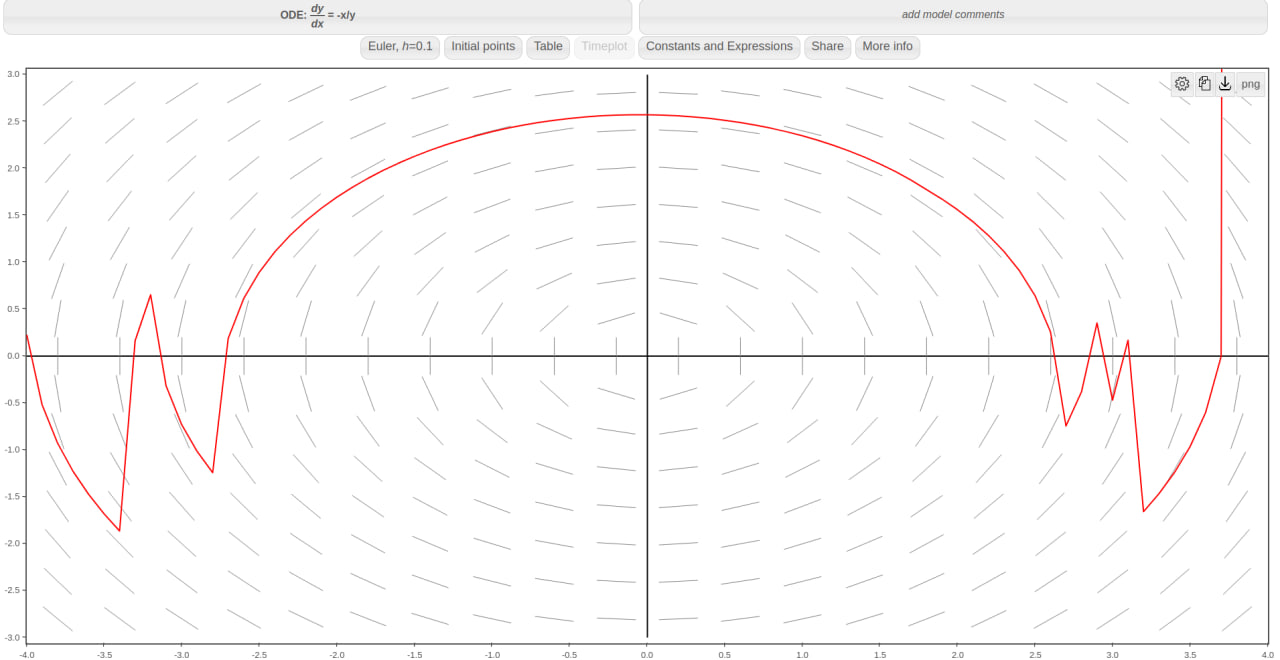
\includegraphics[width=11cm, height=9cm]{web.jpg}
\end{center}

\centerline{\textit{Fig. Error of Euler's method in a popular web application.}} 

\section{Analysis of numerical methods}

To analyze the causes of unreliable differential equations' solutions, the information from science book was applied.  For most of differential equations there are no opportunities to plot an accurate solution. It is the reason, why numerical methods are approached. Using numerical methods allows to solve differential equations only approximately. Value of error rate is not known for advance and many numerical methods do not provide ways of its assessment. That is why it is necessary to know the causes of the errors and to have an ability to estimate quality of a numerical method in a specific case. \\
The topic of solving Cauchy problem using numerical methods was considered with this type of differential equations. 
\begin{myequation}
    \begin{cases}
        $\boldsymbol{\frac{dy}{dx} = f(x,y)}$ \\
        $\boldsymbol{y(x_0) = y_0}$
    \end{cases}
\end{myequation}
Where $x_0$ and $y_0$ are initial conditions.

\vspace{6mm}

\textbf{Cauchy's theorem} If the right-hand side $f(x, y)$ of equation (1) and its partial derivative $\frac{df}{dy}$ are defined and continuous in some domain of variation of variables x and y , then for every inner point $(x_0, y_0)$ of this domain , this equation has a unique solution taking the given value $y = y_0$ when $x = x_0$.

\vspace{6mm}

Numerical methods provide an approximate solution of a differential equation. In this article, Euler's and Runge-Kutta numerical methods are considered. Euler's method is mentioned for studying of numerical methods' errors when it is approached. 
\begin{myequation}
    \centerline{$\boldsymbol{x_{k+1} = x_k + h}$}
\end{myequation}
\begin{myequation}
    \centerline{$\boldsymbol{y_{k+1} = y_k + h f(x_k, y_k)}$}
\end{myequation}

This method is defined for Cauchy problem (1). It was the first numerical method of solving differential equations.




\section{Error's causes of numerical methods}
When differential equations (or systems of equations) are integrated numerically, then differential equation is changed to the corresponding difference equation. While integration, error increases after each step and all errors tend to accumulate. It is called an error of the chosen numerical method's step. Errors, which are made on each step, have the property of accumulating and it leads to the existence of a general integration error $\boldsymbol{\delta_n}$.  \\
\par Therefore, it is observed that two processes become the causes of $\boldsymbol{\delta_n}$ existence.
Firstly, it is the process of an error occurrence. Secondly, it is a process of an error's accumulation.
Let us analyze the process of numerical modelling in Euler's method. It was supposed that all the calculations are made accurately. We could express $\boldsymbol{\delta_{n+1}}$ by $\boldsymbol{\delta_n}$.

\begin{myequation}
    \centerline{$\boldsymbol{\delta_{n+1}} \boldsymbol{=} \boldsymbol{y (x_{n+1}) - y_{n+1}}$}
\end{myequation}
\\
\par From this calculations we can make some conclusions. Firstly, if a step $\boldsymbol{h}$ is too high, then the main cause of an error will be the approximation error $\boldsymbol{e_n}$. However, if $\boldsymbol{h}$ value is low, the approximation error can increase significantly when the process of calculation $\boldsymbol{(x_n , y_n)}$ approaches the area where function $\boldsymbol{f}$ or one of its derivatives $\boldsymbol{\frac{df}{dx}}$, $\boldsymbol{\frac{df}{dy}}$ take unlimited values. Attention should be paid, when $\boldsymbol{h}$ becomes lower, then the approximation error would decrease, but it would never disappear. 
\par It can be observed that the connection between areas of huge errors $\boldsymbol{e_n}$ and areas of violation of sufficient conditions for the existence and uniqueness of a solution in Cauchy's theorem. Indeed, as follows from the Cauchy-Picard theorem, unboundedness of $\boldsymbol{f(x,y)}$ violates a sufficient condition for the existence of a solution $\boldsymbol{y = y(x)}$ and limitlessness of $\boldsymbol{\frac{df}{dy}}$ violates sufficient conditions of its uniqueness.


\subsection{Errors related to unbounded value of a function}
\par Calculation errors of numerical methods are able to affect general accuracy of a solution. Errors of numerical methods has been analyzed for two differential equations and two systems of differential equations.
The first considered equation with incorrect solution of numerical methods (Euler's and Runge-Kutta) was \\
\begin{myequation}
\centerline{$\boldsymbol{\frac{dy}{dx} = - \frac{x}{y}}$}
\end{myequation} \\
If $\boldsymbol{f(x^*, y^*)}$  looses its continuity then perhaps $\boldsymbol{f}$ ceases to be bounded.
The result of solving this equation with Euler's and Runge-Kutta methods demonstrated that when the function tended to zero, then methods could not cope with right calculation of the next step. 
When on the specified step the value of denominator $\boldsymbol{y}$ equals zero, when a numerical methods start to build solution of the differential equation, which has another initial conditions. It happens because  $\boldsymbol{f(x, 0) = \infty}$. 

\includegraphics[width=7cm, height=7cm]{click_circle.png}

\includegraphics[width=7cm, height=7cm]{first_equation.png} 
\centerline{\textit{Fig. Direction field and comparison of numerical and accurate solutions.}}

\vspace{20mm}

A grey circle, which is drawn at the chart, is a limit. It means that a student is able to click only at a field inside the grey circle. This limit has been implemented because if a student would decide to click at a point, which would not be inside the grey circle, he or she would not see the wrong solution of numerical methods (solutions would be the same as accurate). A student is allowed to choose a point inside a grey circle and click on it to observe the behavior of curve, when Euler's and Runge-Kutta methods are approached. Red curve represents Euler's method solution, blue curve illustrates Runge-Kutta method solution and green line is an accurate solution. The green line is a half of a circle.


\subsection{Errors related to unstable gap}
\begin{myequation}
    \centerline{$\boldsymbol{\frac{dy}{dx} = \sqrt{1 - y^2}}$}
\end{myequation}
This function is defined when $\boldsymbol{1 - y^2 \geq 0}$, $\boldsymbol{\lvert y \rvert \le 1}$. From the equation we can get $\boldsymbol{\frac{df}{dy} = \frac{y}{\sqrt{1 - y^2}}}$ and if $\boldsymbol{y = 1}$ or $\boldsymbol{y = -1}$ then $\boldsymbol{\frac{df}{dy}}$ would experience unstable gap. It happens because when $\boldsymbol{y = \pm 1}$ then the denominator of $\boldsymbol{\frac{df}{dy}}$ equals zero.
\par As regards practical part (plots), numerical methods cannot cope with accurate calculation of the next steps when the solution tends to $\pm 1$. It just crosses it and then stops further calculations.
The system was solved manually and then the solving mathematical algorithm was implemented and integrated into the educational application.
\vspace{15mm}
\begin{center}
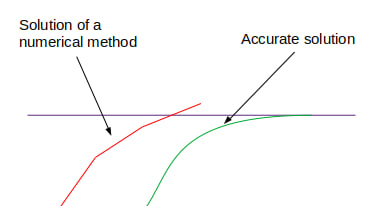
\includegraphics[width=9cm, height=7cm]{paint2.jpg}
\end{center}

\centerline{\textit{Fig. Illustration of numerical method's error. The first equation.}} 

\vspace{15mm}

\begin{center}

\includegraphics[width=7cm, height=7cm]{second_equation.png} 
\end{center}

\centerline{\textit{Fig. Illustration of numerical method's error. The first equation.}} 

\vspace{15mm}

It is observed that numerical methods cannot count all step values, which are defined (51 steps in example). An application shows the number of steps, processed by numerical method. 
Moreover, students have an opportunity to observe the difference between numerical methods' solutions and accurate solutions.


\subsection{Errors associated with growing on each step}
\begin{myequation}
    \begin{cases}
        $\boldsymbol{\frac{dy}{dx} = -x + 2y}$ \\
        $\boldsymbol{\frac{dy}{dx} = -2x + y}$
    \end{cases}
\end{myequation}
 


\vspace{15mm}
This equation was solved with SymPy module then points was generated and the accurate solution was plotted.
According to Euler's method formula:
\subsection{Errors associated with growing on each step}
\begin{myequation}
    \begin{cases}
        $\boldsymbol{\dot{x} = P(x,y)}$ \\
        $\boldsymbol{\dot{y} = Q(x,y)}$
    \end{cases}
\end{myequation}
Euler's method for system of differential equations.
\begin{myequation}
    \begin{cases}
        $\boldsymbol{x_{k+1} = x_k + h P(x_k, y_k)}$ \\
        $\boldsymbol{y_{k+1} = y_k + h Q(x_k, y_k)}$
    \end{cases}
\end{myequation}
where $x_k$ and $y_k$ was current coordinates, $x_{k+1}$ and $y_{k+1}$ was the next coordinates.
\par The problem of this equation was that after each step $h$ a numerical method distanced the line of solution. This error is also called the transfer error to the difference system.
\begin{center}
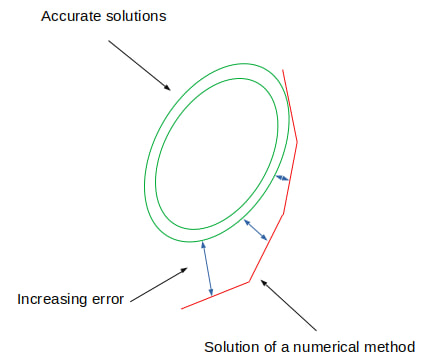
\includegraphics[width=11cm, height=9cm]{paint1.jpg}
\end{center}

\centerline{\textit{Fig. Illustration of increasing error.}} 

\begin{center}
\includegraphics[width=7cm, height=7cm]{first_system.png}
\end{center}
\centerline{\textit{Fig. Comparison of numerical methods and accurate solution for the system.}}

\vspace{15mm}

This figure illustrates the output of the educational application. The red line is a solution of Euler's method. I can be observed that it is wrong and the curve is distanced. As regards Runge-Kutta method it can draw the solution which is the same as accurate but it needs more than five hundred steps. 



\subsection{Errors in nonlinear system (false limit transition)}
Some interesting effects related to numerical integration can be observed in nonlinear systems where features changes significantly when phase trajectories goes from one field of phase space to another. Let us consider nonlinear system.
\vspace{10mm}
\begin{myequation}
    \begin{cases}
        $\boldsymbol{\frac{dy}{dx} = y - ( x^2 + y^2)}$ \\
        $\boldsymbol{\frac{dy}{dx} = -x - y(x^2 + y^2)}$
    \end{cases}
\end{myequation}

\vspace{8mm}


Before approaching numerical methods it was solved manually and algorithm of solving this specific system was implemented and integrated into the application. Method of transition to polar coordinates was approached. The calculations are given lower.
\vspace{10mm}

\begin{myequation}
\centerline{$\boldsymbol{x^2 + y^2 = \rho^2}$}
\end{myequation}

\begin{myequation}
    \begin{cases}
        $\boldsymbol{x = \rho \cos{\theta}}$ \\
        $\boldsymbol{y = \rho \sin{\theta}}$
    \end{cases}
\end{myequation}


\begin{myequation}
    \begin{cases}
        $\boldsymbol{\frac{dx}{dt} = \dot{\rho} \cos{\theta} - \rho\sin{\theta} \dot{\theta}}$\\
        $\boldsymbol{\frac{dy}{dt} = \dot{\rho} \sin{\theta} + \rho \cos{\theta} \dot{\theta}}$
    \end{cases}
\end{myequation}

(12) and (13) was inserted into (10):
\begin{myequation}
    \begin{cases}
        $\boldsymbol{\dot{\rho} \cos{\theta} - \rho \sin{\theta} \dot{\theta} = \rho \sin{\theta} - \rho^2 \rho \cos{\theta}}$\\
        $\boldsymbol{\dot{\rho} \sin{\theta} + \rho \cos{\theta} \dot{\theta} = - \rho \cos{\theta} - \rho^2 \rho \sin{\theta}}$
    \end{cases}
\end{myequation}

The first equation in (14) was multiplied by $\cos{\theta}$ and the second equation was multiplied by $\sin{\theta}$. Then both equations were summarized:
\begin{myequation}
\centerline{$\boldsymbol{\dot{\rho} = - \rho^3}$}
\end{myequation}

\begin{myequation}
\centerline{$\boldsymbol{\int \frac{d\rho}{\rho^3} = -\int dt}$}
\end{myequation}

\begin{myequation}
\centerline{$\boldsymbol{- \frac{1}{2} \rho^{-2} = -t + C}$}
\end{myequation}

Then the first equation in from the system (14) was multiplied by $\sin{\theta}$, the second equation was multiplied by $\cos{\theta}$ and then we subtracted the first equation from the second.
\begin{myequation}
\centerline{$\boldsymbol{\rho \dot{\theta} = -\rho}$}
\end{myequation}

\begin{myequation}
\centerline{$\boldsymbol{\dot{\theta} = -1}$}
\end{myequation}

\begin{myequation}
\centerline{$\boldsymbol{\theta = -t + \theta_0}$}
\end{myequation}
Then
\begin{myequation}
\centerline{$\boldsymbol{\rho = \frac{1}{\sqrt{2t + \frac{1}{\rho_0^2}}}}$}
\end{myequation}
Therefore, while the process of numerical integration was executed, the system of differential equations experienced false limit transition, which it did not have in accurate solution.
It is essential to mention that this effect with the error was caused not because of a numerical method but because of lack of system's roughness.
\par Actually, the accurate solution was a spiral and the application demonstrated the difference between numerical methods' solutions and the accurate solution.

\vspace{10mm}

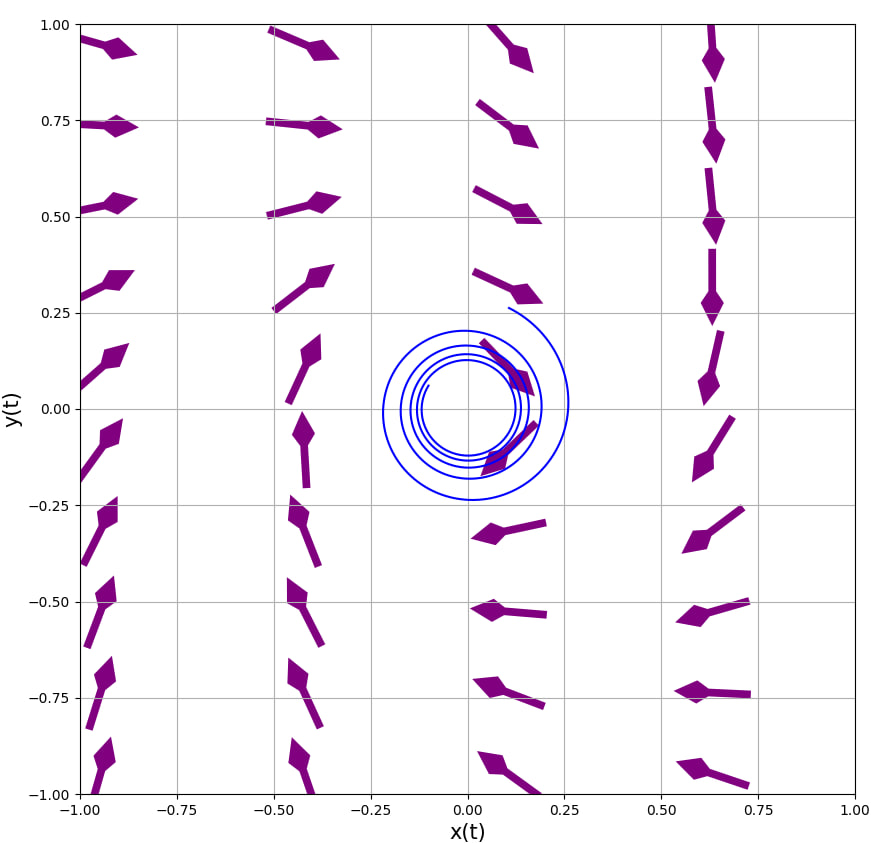
\includegraphics[width=7cm, height=7cm]{runge_cycle.jpg}
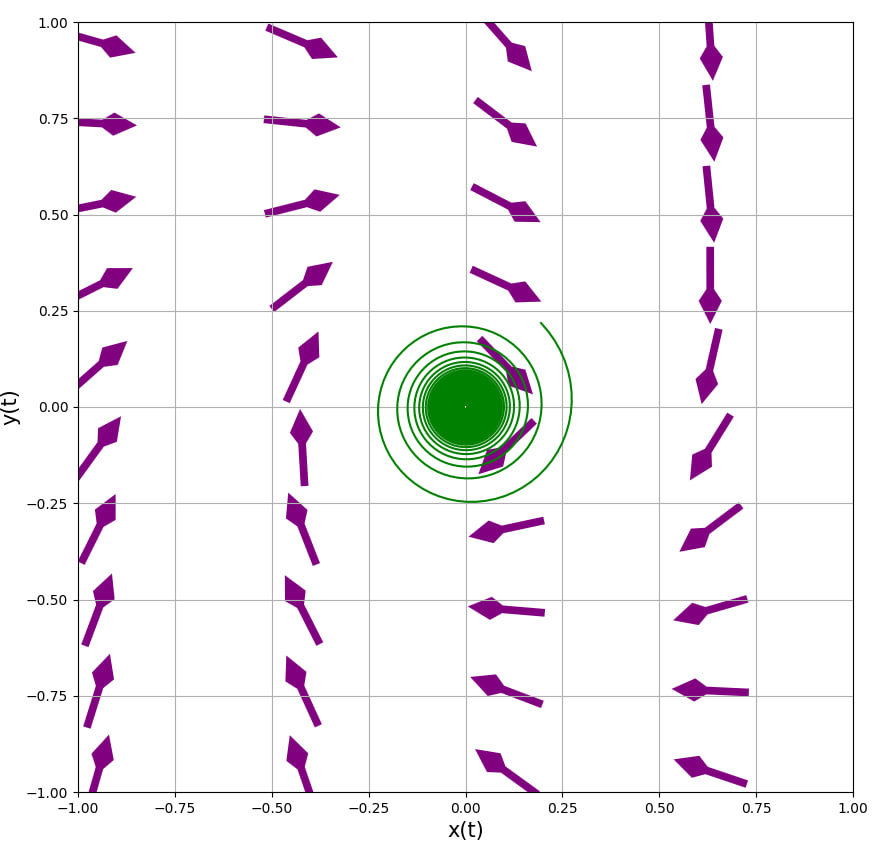
\includegraphics[width=7cm, height=7cm]{green_cycle.jpg} 
\centerline{\textit{Fig. Direction field and comparison of numerical and accurate solutions.}}

\vspace{15mm}


It can be observed that Runge-Kutta method's solution has a false limit transition and the accurate solution goes right to zero. Students are able to see it using the educational application.








\section{Educational application for comparison of numerical solutions of DEs and its accurate solution}
To demonstrate, how numerical solutions of differential equations can lead to mistakes and disinformation. There are several types of incorrect differential equations' solutions, which are considered in this paper.
Two numerical methods have been integrated inside the application: Euler's and Runge-Kutta. Students would have an oppurtunity to compare both of them. Moreover, to draw an accurate solution of a differential equation, SymPy module has been approached.  
\subsection{Interface of the application}
The graphical user application consists of buttons to choose the equation, that a student would like to analyze and green button with information (to be familiar with ways of using the application). The next window allows an user to define the number of steps for both Euler's and Runge-Kutta methods. \\
A student would be able to choose the equation he/she would like to analyze.

\vspace{10mm}

\begin{center}
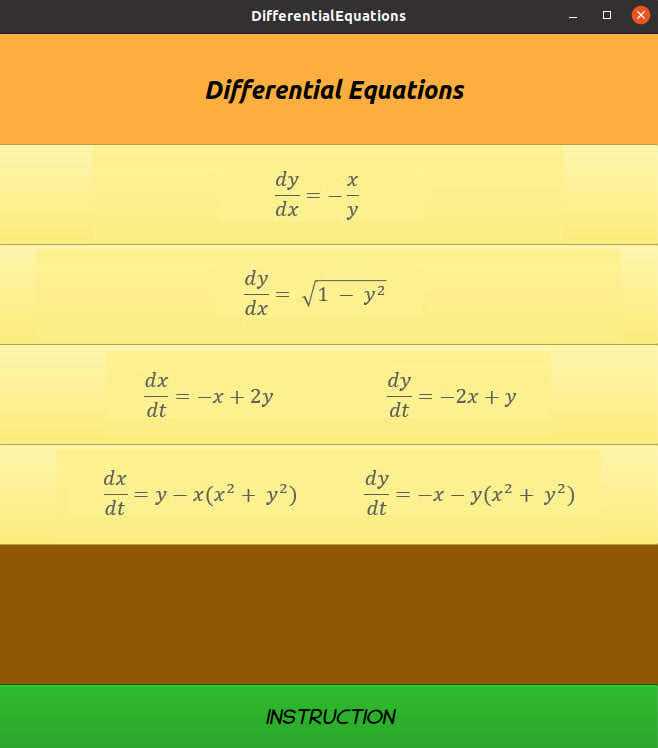
\includegraphics[width=7cm, height=8cm]{menu.jpg}
\end{center}

\centerline{\textit{Fig. Menu of the application.}} 

\vspace{15mm}

After executing the application student would have a list of differential equations and he/she should choose the equation for analysis and click on it. Furthermore, it is necessary to click on "Instruction" button to be familiar with a program interface before usage (to avoid misunderstandings).

\vspace{15mm}

\begin{center}
\includegraphics[width=9cm, height=7cm]{inst.jpg}
\end{center}

\centerline{\textit{Fig. Instruction of the application.}} 

\vspace{15mm}

Instruction contains information about the application's use cases (what mouse and keyboard buttons students should click to observe solutions).

\vspace{15mm}

\begin{center}
\includegraphics[width=7cm, height=7cm]{parameters.png}
\end{center}

\centerline{\textit{Fig. Window to specify the number of steps.}} 

\vspace{15mm}

\par After clicking 'Continue' button, a student would have an opportunity to click at a chart (the click point is an initial condition for the differential equation).\\

\subsection{Methodology}
\par Matplotlib module, which is integrated in Python gave an opportunity to solve Cauchy problem just clicking at the point. It draws the solutions of numerical methods (Euler's and Runge-Kutta) and accurate solutions to compare. Matplotlib module lets define the behavior of charts when buttons of mouse or keybord are clicked.
\par It was described that SymPy module helped to plot some solutions of differential equations and then generate points. However, it cannot cope with nonlinear differential equations. That is why some of equations were solved manually.
\par Approximately 1500 lines of code were written to implement this program. The development was made in Visual Studio code. The operating system, where development was made, was Ubuntu 20.04. 
After the end of the application's implementation it was necessary to make an executable file. It would give an opportunity to users to use this program without installing Python and PyQT5. To do this "auto-py-to-exe" program was approached and executable file was generated both for Windows and Linux operating systems.

\section{Conclusion}
To sum up, two differential equations and two systems of differential equations have been analyzed in this work. Four types of errors, when numerical methods are approached for solving differential equations, have been described and analyzed. 
\par To check if numerical methods' solutions are wrong, the application with graphical user interface has been implemented. To draw accurate solutions SymPy module and algorithms based on manual decisions have been obtained. The main conclusion of the work was to analyze differential equations manually and not to always trust numerical methods as sometimes it made students be confused. The application, which was implemented for this research, would give students an opportunity to compare numerical methods' solution with accurate solution. The main message of this paper is to use manual analysis of differential equations before using numerical methods as sometimes they should not be trusted. 








\newpage
\addcontentsline{toc}{section}{\bf{References}}
\renewcommand\refname{References}
\begin{thebibliography}{99}
\bibitem{Gor}{\sl Gorodetsiy S. Yu., Kotova T. A., Skornyakova B. L., Hentov A. A.} Solving differential equations by numerical methods such as the progress of mathematical simulations~//{\it Lab. Features of numerical modeling of solutions of differential equations}, 2001. 

\end{thebibliography}

[2] Official web site of SymPy module https://docs.sympy.org/latest/modules/solvers/ode.html
\vspace{1mm}

[3] Official web site of Matplotlib module https://matplotlib.org
\end{document}
